\UseRawInputEncoding
% Plan du rapport individuel NaturaCorp (version avancee)

% ===================
% Preambule avance
% ===================

\documentclass[a4paper,12pt]{report}

% Numérotation personnalisée
\renewcommand{\thesection}{\arabic{section}}
\renewcommand{\thesubsection}{\thesection.\arabic{subsection}}

% Packages principaux
\usepackage[french]{babel}
\usepackage[utf8]{inputenc}
\usepackage[T1]{fontenc}
\usepackage{graphicx}
\usepackage{xcolor}
\usepackage{geometry}
\usepackage{titlesec}
\usepackage{array}
\usepackage{longtable}
\usepackage{booktabs}
\usepackage{caption}
\usepackage{hyperref}
\usepackage[most]{tcolorbox}
\usepackage{tikz}
\usepackage{listings}
\usepackage{enumitem}

% Configuration des liens hypertextes
\definecolor{naturacorpgreen}{RGB}{0,128,64}
\hypersetup{
    colorlinks=true,
    linkcolor=naturacorpgreen,
    urlcolor=blue,
    citecolor=blue,
    pdftitle={Rapport Individuel - NaturaCorp},
    pdfauthor={À compléter},
    pdfsubject={Documentation de maintenance évolutive},
    pdfkeywords={NaturaCorp, Maintenance, Évolution, Rapport},
    pdfstartview={FitH},
    bookmarksnumbered=true,
    pdfpagemode=UseOutlines
}

% Mise en page
\geometry{margin=2.5cm}

% Couleurs personnalisées
\definecolor{lightgray}{HTML}{F2F2F2}
\definecolor{codegreen}{rgb}{0,0.6,0}
\definecolor{codegray}{rgb}{0.5,0.5,0.5}
\definecolor{codepurple}{rgb}{0.58,0,0.82}
\definecolor{backcolour}{rgb}{0.95,0.95,0.92}

% Personnalisation des titres
\titleformat{\section}
  {\normalfont\Large\bfseries\color{naturacorpgreen}}
  {\thesection}{1em}{}
\titleformat{\subsection}
  {\normalfont\large\bfseries}
  {\thesubsection}{1em}{}

% En-tête et pied de page
\usepackage{fancyhdr}
\fancyhf{}
\fancyfoot[L]{Juin 2025}
\fancyfoot[C]{NaturaCorp - Maintenance évolutive}
\fancyfoot[R]{\thepage}
\renewcommand{\footrulewidth}{0.4pt}
\pagestyle{fancy}

% ===================
% Début du document
% ===================
\begin{document}

% --- PAGE DE GARDE ---
\thispagestyle{empty}
\begin{center}
    \begin{minipage}{0.45\textwidth}
        \centering
        \includegraphics[width=5cm]{naturacorp.png}
        \vspace{0.3cm}
    \end{minipage}
    \hfill
    \begin{minipage}{0.45\textwidth}
        \centering
        \includegraphics[width=5cm]{esn.jpeg}
        \vspace{0.3cm}
    \end{minipage}
    \vspace*{0.5cm}
    
    % Titre principal
    {\Huge\bfseries\color{naturacorpgreen} Rapport Individuel -- Projet NaturaCorp\par}
    \vspace{1.2cm}
    
    % Sous-titre
    {\LARGE\bfseries Livrable 4.3 -- Maintenance évolutive\par}
    \vspace{2cm}
    
    % Auteur
    {\Large\bfseries Réalisé par :\par}
    \vspace{0.3cm}
    {\Large SELLIER Luka\par}
    \vspace{0.5cm}
    {\large Formation : Bachelor 3 Développement WEB\par}
    \vspace{0.3cm}
    \vspace{0.3cm}
    {\large Année universitaire : 2024--2025\par}
    \vspace{1.5cm}
    
    % Informations projet
    \begin{minipage}{0.8\textwidth}
        \centering
        \textbf{Projet d'évolution fonctionnelle}%
        \vspace{0.2cm}
        Maintenance évolutive de la solution numérique NaturaCorp
    \end{minipage}
    \vspace{1.5cm}
    
    % Date
    {\large Juin 2025\par}
\vspace*{\fill}
\begin{center}
    \textbf{Livrable 4.3 : Maintenance évolutive}
\end{center}
\end{center}

\newpage
% --- SOMMAIRE ---
\renewcommand{\contentsname}{Sommaire}
\tableofcontents
\newpage

\section{Introduction}
  \subsection{Contexte du projet et de la roadmap}
  Dans le cadre du livrable 4.3 de maintenance évolutive du projet NaturaCorp, j'ai été chargé d'implémenter de nouvelles fonctionnalités visant à améliorer l'expérience utilisateur et à enrichir les capacités d'analyse des données pour les commerciaux et les administrateurs. NaturaCorp est une entreprise spécialisée dans la distribution de produits naturels aux pharmacies, et sa plateforme numérique joue un rôle crucial dans la gestion des relations commerciales et l'analyse des performances.

  La roadmap du projet prévoyait plusieurs évolutions fonctionnelles pour cette phase, notamment l'enrichissement du tableau de bord commercial avec des visualisations graphiques et des fonctionnalités d'export, ainsi que l'amélioration de la page "Rapports" pour les administrateurs avec des capacités d'analyse et d'export plus avancées.

  \subsection{Objectifs de la fonctionnalité choisie}
  Pour ce livrable, j'ai choisi de me concentrer sur l'implémentation des fonctionnalités suivantes :
  
  \begin{itemize}
    \item Afficher sous forme de graphique le nombre de ventes du commercial sur une période donnée
    \item Afficher sous forme de graphique la liste des clients rapportés par le commercial sur une période donnée
    \item Permettre le téléchargement en CSV séparé de chaque graphique ou tableau de données
    \item Enrichir la page "Rapports" avec des fonctionnalités d'export CSV pour les tableaux de pharmacies par zone et de performances des commerciaux
    \item Ajouter des visualisations graphiques pour la répartition des pharmacies et des commandes par zone et par commercial
  \end{itemize}
  
  Ces fonctionnalités visent à fournir aux utilisateurs des outils d'analyse visuelle plus puissants et à faciliter l'exploitation des données en permettant leur export dans un format standard. L'objectif principal est d'améliorer la prise de décision basée sur les données et de renforcer le suivi des performances commerciales.

\newpage 
\section{Analyse préalable}
  \subsection{Enjeux fonctionnels, techniques ou utilisateurs}
  L'analyse préalable du projet a permis d'identifier plusieurs enjeux majeurs :
  
  \begin{itemize}
    \item \textbf{Enjeux fonctionnels} : Les commerciaux avaient besoin d'une visualisation claire de leurs performances de vente et de leur capacité à acquérir de nouveaux clients. De même, les administrateurs nécessitaient une vue d'ensemble plus détaillée de la répartition des pharmacies par zone et des performances des commerciaux, avec la possibilité d'exporter ces données pour une analyse plus approfondie.
    
    \item \textbf{Enjeux techniques} : L'implémentation de graphiques interactifs nécessitait l'intégration d'une bibliothèque JavaScript adaptée (Chart.js) et la création d'un contrôleur dédié pour la préparation et la structuration des données. La génération de fichiers CSV devait être optimisée pour gérer efficacement de grands volumes de données sans impact sur les performances du serveur.
    
    \item \textbf{Enjeux utilisateurs} : L'interface utilisateur devait rester intuitive malgré l'ajout de nouvelles fonctionnalités. Les graphiques devaient être lisibles et informatifs, avec une granularité adaptée à la période sélectionnée. Les exports CSV devaient contenir toutes les informations pertinentes tout en restant faciles à exploiter dans des outils d'analyse externes.
  \end{itemize}

  \subsection{Contraintes identifiées}
  Plusieurs contraintes ont été identifiées lors de l'analyse préalable :
  
  \begin{itemize}
    \item \textbf{Contraintes techniques} : 
    \begin{itemize}
      \item Nécessité de maintenir la compatibilité avec l'architecture MVC existante de Laravel
      \item Gestion des requêtes SQL complexes pour l'agrégation des données sans impact sur les performances
      \item Adaptation de l'interface utilisateur aux différentes tailles d'écran pour garantir la lisibilité des graphiques
      \item Résolution des problèmes d'ambiguïté dans les requêtes SQL impliquant plusieurs tables avec des noms de colonnes identiques
    \end{itemize}
    
    \item \textbf{Contraintes fonctionnelles} : 
    \begin{itemize}
      \item Nécessité d'adapter la granularité des données (jour, semaine, mois) en fonction de la période sélectionnée
      \item Cohérence entre les données affichées dans les graphiques et celles exportées en CSV
      \item Gestion des périodes de temps (30 derniers jours, 3 derniers mois, etc.) de manière précise et cohérente
    \end{itemize}
    
    \item \textbf{Contraintes d'intégration} : 
    \begin{itemize}
      \item Respect de la charte graphique existante et de l'expérience utilisateur globale
      \item Intégration harmonieuse des nouveaux éléments d'interface dans les pages existantes
    \end{itemize}
  \end{itemize}

\section{Conception}
  \subsection{Schéma de base de données \(si applicable\)}
  Pour ce projet de maintenance évolutive, aucune modification du schéma de base de données n'a été nécessaire. Les fonctionnalités développées s'appuient sur les structures de données existantes :
  
  \begin{itemize}
    \item Table \texttt{orders} : Stockage des commandes avec les informations de base (date, montant, statut)
    \item Table \texttt{order\_items} : Détails des articles commandés (quantité, prix unitaire, remise)
    \item Table \texttt{pharmacies} : Informations sur les pharmacies clientes (nom, adresse, zone, commercial assigné)
    \item Table \texttt{users} : Utilisateurs du système, incluant les commerciaux
    \item Table \texttt{zones} : Zones géographiques pour l'organisation des pharmacies
  \end{itemize}
  
  Les relations existantes entre ces tables ont été exploitées pour générer les données nécessaires aux graphiques et aux exports CSV.

  \subsection{Diagrammes ou maquettes \(si utiles à la compréhension\)}
  Bien que des maquettes détaillées n'aient pas été nécessaires pour ce projet, voici une représentation conceptuelle des éléments ajoutés :
  
  \begin{tcolorbox}[colback=lightgray!10!white, colframe=naturacorpgreen, title=Structure du tableau de bord commercial]
  \begin{itemize}
    \item En-tête avec sélecteur de période (30 derniers jours, 3 derniers mois, 6 derniers mois, dernière année)
    \item Graphique des ventes avec bouton d'export CSV
    \item Graphique des clients rapportés avec bouton d'export CSV
    \item Tableau des commandes récentes
  \end{itemize}
  \end{tcolorbox}
  
  \begin{tcolorbox}[colback=lightgray!10!white, colframe=naturacorpgreen, title=Structure de la page Rapports administrateur]
  \begin{itemize}
    \item Statistiques synthétiques (zone et commercial les plus performants)
    \item Tableau des pharmacies par zone avec boutons d'export CSV (global et par zone)
    \item Tableau des performances des commerciaux avec boutons d'export CSV (global et par commercial)
    \item Graphiques de répartition des pharmacies et des commandes par zone
    \item Graphiques de répartition des pharmacies et des commandes par commercial
  \end{itemize}
  \end{tcolorbox}

\newpage
  \subsection{Choix techniques argumentés}
  Plusieurs choix techniques ont été effectués pour garantir la qualité et la maintenabilité de la solution :
  
  \begin{itemize}
    \item \textbf{Chart.js pour les visualisations graphiques} : Cette bibliothèque JavaScript a été choisie pour sa légèreté, sa simplicité d'intégration et sa richesse fonctionnelle. Elle offre une grande variété de types de graphiques (lignes, barres, camemberts) et des fonctionnalités interactives comme les infobulles au survol.
    
    \item \textbf{Contrôleur dédié pour les exports CSV} : La création d'un contrôleur spécifique (\texttt{ExportController.php}) permet de centraliser la logique d'export et de faciliter la maintenance. Cette approche respecte le principe de responsabilité unique et s'intègre parfaitement dans l'architecture MVC de Laravel.
    
    \item \textbf{Méthode helper pour la gestion des périodes} : L'implémentation d'une méthode \texttt{setPeriodDates()} permet de standardiser le calcul des dates de début et de fin en fonction du type de période sélectionné, garantissant ainsi la cohérence entre l'affichage et l'export des données.
    
    \item \textbf{Granularité adaptative des données} : Le choix d'adapter automatiquement la granularité des données (jour, semaine, mois) en fonction de la durée de la période sélectionnée permet d'optimiser la lisibilité des graphiques et la pertinence des informations affichées.
    
    \item \textbf{Utilisation de Tailwind CSS} : Le framework CSS déjà présent dans le projet a été exploité pour garantir une intégration visuelle cohérente des nouveaux éléments d'interface.
  \end{itemize}

\newpage
\section{Réalisation}
  \subsection{Développement effectué}
  Le développement des fonctionnalités a été réalisé selon une approche méthodique structurée. Pour garantir un suivi rigoureux et une organisation optimale du projet, j'ai mis en place :
  
  \begin{itemize}
    \item \textbf{Un dépôt Git} pour le versionnement complet du code, permettant de suivre l'évolution des modifications et de sécuriser le développement
    
    \item \textbf{Un fichier de contexte} décrivant en détail les objectifs du projet, les contraintes techniques et les fonctionnalités attendues
    
    \item \textbf{Un journal d'avancées} mis à jour régulièrement pour documenter la progression, les décisions prises et les difficultés rencontrées
    
    \item \textbf{Une structure de projet claire} organisant le code selon l'architecture MVC de Laravel
  \end{itemize}
  
  \begin{tcolorbox}[colback=lightgray!50,colframe=naturacorpgreen!75,title=\textbf{Note},fonttitle=\bfseries,coltitle=white,boxrule=0.5mm,arc=3mm]
    Le fichier de contexte et le journal d'avancées sont inclus dans les annexes du Git pour permettre de suivre en détail l'ensemble de la démarche projet. Le code complet du projet sera également sur Git : \href{https://github.com/Kauluche/4.3.nc.1xprod.com}{github.com/Kauluche/4.3.nc.1xprod.com}
  \end{tcolorbox}
  
  Cette approche méthodologique a permis d'assurer la qualité du code et la traçabilité des développements tout au long du projet. Voici les principales étapes techniques du développement :
  
  \begin{enumerate}
    \item \textbf{Création du contrôleur d'export} : Développement du fichier \texttt{ExportController.php} avec les méthodes nécessaires pour générer les exports CSV des différentes données (ventes, clients, pharmacies par zone, performances des commerciaux).
    
    \item \textbf{Ajout des routes d'export} : Configuration des routes dans \texttt{routes/web.php} pour accéder aux différentes fonctionnalités d'export CSV.
    
    \item \textbf{Modification du contrôleur du tableau de bord} : Enrichissement du \texttt{DashboardController.php} avec les méthodes de préparation des données pour les graphiques (\texttt{prepareSalesChartData} et \texttt{prepareClientsChartData}).
    
    \item \textbf{Intégration des graphiques} : Ajout de Chart.js et implémentation des graphiques dans les vues \texttt{dashboard.blade.php} et \texttt{admin/reports/index.blade.php}.
    
    \item \textbf{Correction de bugs} : Résolution d'un problème d'ambiguïté SQL dans les requêtes impliquant plusieurs tables avec des colonnes de même nom.
    
    \item \textbf{Amélioration de l'interface utilisateur} : Optimisation de la mise en page et du style des graphiques et boutons d'export pour une meilleure expérience utilisateur.
    
    \item \textbf{Ajout de statistiques synthétiques} : Enrichissement de la page des rapports administrateur avec des blocs de statistiques sur les zones et commerciaux les plus performants.
  \end{enumerate}

  \subsection{Captures de code ou extraits clés avec explication}

    \begin{tcolorbox}[colback=lightgray,colframe=naturacorpgreen,title=\textbf{Information complémentaire},fonttitle=\bfseries,coltitle=white]
    Des rapports détaillés sur chacune des fonctionnalités clés développées ont été joints en annexe. Ces documents techniques fournissent davantage de détails sur le code et l'implémentation si cela vous intéresse.
  \end{tcolorbox}
  
  Voici quelques extraits de code clés qui illustrent les aspects importants du développement :
  
  \begin{lstlisting}[caption=Méthode prepareSalesChartData dans DashboardController.php]
  private function prepareSalesChartData($user, Carbon $startDate, Carbon $endDate)
  {
      $pharmacyIds = $user->pharmacies()->pluck('id')->toArray();
      
      $salesData = [];
      $labels = [];
      $interval = 'month'; // Par defaut, intervalle mensuel
      
      // Determiner l'intervalle approprie en fonction de la duree
      $diffInDays = $startDate->diffInDays($endDate);
      
      if ($diffInDays <= 31) {
          // Periode courte (moins d'un mois) : afficher par jour
          $interval = 'day';
      } else if ($diffInDays <= 90) {
          // Periode moyenne (1-3 mois) : afficher par semaine
          $interval = 'week';
      }
      
      // Generation des donnees selon l'intervalle approprie
      $currentDate = clone $startDate;
      
      while ($currentDate <= $endDate) {
          // Code pour generer les donnees selon l'intervalle...
          // ...
      }
      
      return [
          'labels' => $labels,
          'data' => $salesData
      ];
  }
  \end{lstlisting}
  
  Cet extrait montre comment la granularité des données est adaptée automatiquement en fonction de la durée de la période sélectionnée, ce qui permet d'optimiser la lisibilité des graphiques.
  
  \begin{lstlisting}[caption=Méthode d'export CSV dans ExportController.php]
  public function exportCommercialSales(Request $request)
  {
      $user = Auth::user();
      
      // Utilisation de la methode helper pour definir les dates
      list($startDate, $endDate) = $this->setPeriodDates($request);
      
      $pharmacyIds = $user->pharmacies()->pluck('id')->toArray();
      
      // Requete pour recuperer les ventes
      $sales = Order::whereIn('pharmacy_id', $pharmacyIds)
          ->whereDate('orders.created_at', '>=', $startDate)
          ->whereDate('orders.created_at', '<=', $endDate)
          ->join('order_items', 'orders.id', '=', 'order_items.order_id')
          ->join('pharmacies', 'orders.pharmacy_id', '=', 'pharmacies.id')
          ->select(
              'orders.id',
              'pharmacies.name as pharmacy_name',
              'orders.created_at',
              DB::raw('SUM(order_items.quantity * order_items.unit_price * (1 - order_items.discount_percentage / 100)) as total_amount')
          )
          ->groupBy('orders.id', 'pharmacies.name', 'orders.created_at')
          ->orderBy('orders.created_at', 'desc')
          ->get();
      
      // Generation du CSV
      $filename = 'ventes_' . $startDate->format('Y-m-d') . '_' . $endDate->format('Y-m-d') . '.csv';
      
      $headers = [
          'Content-Type' => 'text/csv; charset=UTF-8',
          'Content-Disposition' => 'attachment; filename="' . $filename . '"',
      ];
      
      $callback = function() use ($sales) {
          $file = fopen('php://output', 'w');
          
          // En-tetes CSV
          fputcsv($file, ['ID', 'Pharmacie', 'Date', 'Montant total (EUR)']);
          
          // Donnees
          foreach ($sales as $sale) {
              fputcsv($file, [
                  $sale->id,
                  $sale->pharmacy_name,
                  $sale->created_at->format('d/m/Y'),
                  number_format($sale->total_amount, 2, ',', ' ')
              ]);
          }
          
          fclose($file);
      };
      
      return response()->stream($callback, 200, $headers);
  }
  \end{lstlisting}
  
  Cet extrait illustre la méthode d'export des ventes d'un commercial au format CSV, avec la récupération des données pertinentes et leur formatage approprié.

  \subsection{Difficultés rencontrées et gestion}
  Plusieurs difficultés ont été rencontrées lors du développement et ont été résolues de manière méthodique :
  
  \begin{itemize}
    \item \textbf{Problème d'ambiguïté SQL} : Une erreur "Integrity constraint violation: 1052 Column 'created\_at' in where clause is ambiguous" a été identifiée dans le \texttt{DashboardController.php}. Cette erreur était due à l'ambiguïté de la colonne \texttt{created\_at} présente dans les tables \texttt{orders} et \texttt{order\_items}. La solution a consisté à spécifier explicitement la table dans les clauses WHERE (\texttt{orders.created\_at} au lieu de \texttt{created\_at}).
    
    \item \textbf{Problème d'affichage des graphiques comprimés} : Les graphiques apparaissaient comprimés et peu lisibles sur certaines tailles d'écran. Ce problème a été résolu en modifiant les conteneurs de graphiques pour qu'ils prennent 100\% de la largeur et en ajoutant des classes CSS personnalisées pour les conteneurs et les éléments canvas. Un script JavaScript a également été implémenté pour ajuster dynamiquement la taille des graphiques au chargement et au redimensionnement.
    
    \item \textbf{Incohérence dans le calcul des périodes} : Une incohérence a été détectée dans le calcul de la période "3 derniers mois" qui couvrait en réalité 4 mois. La correction a consisté à modifier \texttt{subMonths(3)} par \texttt{subMonths(2)} pour couvrir exactement 3 mois (mois courant + 2 mois précédents).
    
    \item \textbf{Synchronisation entre affichage et export} : Pour garantir que les données exportées correspondent exactement à celles affichées dans les graphiques, une méthode helper \texttt{setPeriodDates()} a été créée pour calculer les dates de début et de fin en fonction du type de période. Les liens d'export CSV ont également été mis à jour pour transmettre les paramètres de période actuellement sélectionnée.
  \end{itemize}

\newpage
\section{Tests et validation}
  \subsection{Scénarios de tests mis en place}
  Pour garantir le bon fonctionnement des fonctionnalités développées, plusieurs scénarios de tests ont été mis en place :
  
  \begin{enumerate}
    \item \textbf{Test des graphiques du tableau de bord commercial} :
    \begin{itemize}
      \item Vérification de l'affichage correct des graphiques pour différentes périodes (30 derniers jours, 3 derniers mois, 6 derniers mois, dernière année)
      \item Contrôle de la cohérence des données affichées avec les données présentes en base
      \item Test de l'adaptation automatique de la granularité des données selon la période sélectionnée
      \item Vérification des infobulles au survol des points du graphique
    \end{itemize}
    
    \item \textbf{Test des exports CSV} :
    \begin{itemize}
      \item Vérification de la génération correcte des fichiers CSV pour chaque type d'export
      \item Contrôle de la cohérence des données exportées avec celles affichées dans l'interface
      \item Test des en-têtes et du formatage des données dans les fichiers CSV
      \item Vérification de la gestion des caractères spéciaux et des accents
    \end{itemize}
    
    \item \textbf{Test des graphiques de la page Rapports administrateur} :
    \begin{itemize}
      \item Vérification de l'affichage correct des graphiques circulaires et à barres
      \item Contrôle de la cohérence des données affichées avec les tableaux correspondants
      \item Test des légendes et des infobulles au survol
    \end{itemize}
    
  \end{enumerate}

  \subsection{Résultats observés}
  Les tests ont permis de valider le bon fonctionnement des fonctionnalités développées et d'identifier quelques points d'amélioration qui ont été corrigés :
  
  \begin{itemize}
    \item \textbf{Graphiques du tableau de bord commercial} :
    \begin{itemize}
      \item Les graphiques s'affichent correctement pour toutes les périodes testées
      \item La granularité s'adapte automatiquement selon la période (jour, semaine, mois)
      \item Les données affichées correspondent bien aux données en base
      \item Les infobulles au survol affichent correctement les valeurs précises
    \end{itemize}
    
    \item \textbf{Exports CSV} :
    \begin{itemize}
      \item Les fichiers CSV sont générés correctement pour tous les types d'export
      \item Les données exportées sont cohérentes avec celles affichées dans l'interface
      \item Les en-têtes et le formatage des données sont corrects
      \item Les caractères spéciaux et les accents sont bien gérés grâce à l'encodage UTF-8
    \end{itemize}
    
    \item \textbf{Graphiques de la page Rapports administrateur} :
    \begin{itemize}
      \item Les graphiques circulaires et à barres s'affichent correctement
      \item Les données affichées sont cohérentes avec les tableaux correspondants
      \item Les légendes et les infobulles au survol fonctionnent correctement
    \end{itemize}
    
  \end{itemize}

  \subsection{Outils utilisés \(Postman, Lighthouse, etc.\)}
  Plusieurs outils ont été utilisés pour faciliter le développement, les tests et la validation des fonctionnalités :
  
  \begin{itemize}
    \item \textbf{Git} : Système de contrôle de version pour suivre les modifications et gérer le code source
    
    \item \textbf{Chrome DevTools} : Pour inspecter et déboguer le code HTML, CSS et JavaScript, ainsi que pour tester la responsivité sur différentes tailles d'écran
    
    \item \textbf{Laravel Debugbar} : Extension Laravel pour surveiller les requêtes SQL, les temps de chargement et la consommation de mémoire
    
    \item \textbf{Postman} : Pour tester les routes d'API et les exports CSV en dehors du navigateur
    
    \item \textbf{Lighthouse} : Pour évaluer les performances, l'accessibilité et les bonnes pratiques de développement web
    
    \item \textbf{Excel/LibreOffice Calc} : Pour vérifier la lisibilité et la cohérence des fichiers CSV exportés

  \end{itemize}

\section{Procédure de mise à jour}
  \subsection{Liste des fichiers modifiés}
  Voici la liste complète des fichiers créés ou modifiés dans le cadre de cette maintenance évolutive :
  
  \begin{itemize}
    \item \textbf{Fichiers créés :}
    \begin{itemize}
      \item \texttt{app/Http/Controllers/ExportController.php} : Nouveau contrôleur pour gérer tous les exports CSV
    \end{itemize}
    
    \item \textbf{Fichiers modifiés :}
    \begin{itemize}
      \item \texttt{app/Http/Controllers/Admin/ReportController.php} : Ajout des statistiques synthétiques et des données pour les graphiques
      \item \texttt{app/Http/Controllers/DashboardController.php} : Préparation des données pour les graphiques et correction du bug SQL
      \item \texttt{resources/views/admin/reports/index.blade.php} : Ajout des graphiques, des statistiques et des boutons d'export
      \item \texttt{resources/views/dashboard.blade.php} : Ajout des graphiques et des boutons d'export CSV
      \item \texttt{routes/web.php} : Ajout des routes pour les exports CSV
    \end{itemize}
  \end{itemize}

\newpage
  \subsection{Étapes nécessaires pour intégrer la fonctionnalité dans le projet existant}
  Pour intégrer ces fonctionnalités dans le projet existant, suivez ces étapes :
  
  \begin{enumerate}
    \item \textbf{Sauvegarde préalable} : Effectuez une sauvegarde complète du projet et de la base de données avant toute modification.
    
    \item \textbf{Mise à jour des fichiers} : Copiez les fichiers créés et modifiés dans leurs emplacements respectifs dans la structure du projet.
    
    \item \textbf{Vérification des routes} : Assurez-vous que les nouvelles routes définies dans \texttt{routes/web.php} ne créent pas de conflits avec des routes existantes.
    
    \item \textbf{Intégration de Chart.js} : Si Chart.js n'est pas déjà intégré dans le projet, ajoutez le script CDN dans les vues concernées ou installez-le via npm.
    
    \item \textbf{Vérification des permissions} : Assurez-vous que les utilisateurs ont les permissions nécessaires pour accéder aux nouvelles fonctionnalités (notamment les exports CSV).
    
    \item \textbf{Nettoyage du cache} : Exécutez les commandes Laravel pour nettoyer le cache des routes, des vues et de la configuration.
    
    \item \textbf{Tests} : Exécutez les scénarios de tests décrits précédemment pour vérifier le bon fonctionnement des fonctionnalités.
  \end{enumerate}

  \subsection{Commandes à exécuter si des dépendances ont été ajoutées}
  Aucune dépendance PHP supplémentaire n'a été ajoutée pour ce projet. Cependant, pour garantir le bon fonctionnement de l'application après la mise à jour, exécutez les commandes suivantes :
  
  \begin{lstlisting}[language=bash]
  # Nettoyer le cache des routes
  php artisan route:cache
  
  # Nettoyer le cache des vues
  php artisan view:clear
  
  # Nettoyer le cache de configuration
  php artisan config:clear
  
  # Optimiser l'autoloader de Composer
  composer dump-autoload -o
  \end{lstlisting}
  
  Si vous choisissez d'installer Chart.js via npm plutôt que d'utiliser le CDN, exécutez également ces commandes :
  
  \begin{lstlisting}[language=bash]
  # Installer Chart.js
  npm install chart.js
  
  # Compiler les assets
  npm run dev
  \end{lstlisting}

  \subsection{Précisions sur l'installation ou la mise à jour éventuelle de la base de données}
  Cette maintenance évolutive n'a pas nécessité de modifications du schéma de la base de données. Aucune migration ou mise à jour de la base de données n'est donc requise.
  
  Les fonctionnalités développées s'appuient uniquement sur les structures de données existantes et les relations déjà établies entre les tables \texttt{orders}, \texttt{order\_items}, \texttt{pharmacies}, \texttt{users} et \texttt{zones}.

\section{Bilan personnel}
  \subsection{Apports de cette épreuve}
  Cette épreuve de maintenance évolutive m'a apporté de nombreux enseignements et compétences :
  
  \begin{itemize}
    \item \textbf{Approfondissement de Laravel} : J'ai pu approfondir ma maîtrise du framework Laravel, notamment dans la gestion des requêtes SQL complexes, l'optimisation des performances et la structuration du code selon le pattern MVC.
    
    \item \textbf{Intégration de bibliothèques JavaScript} : L'utilisation de Chart.js m'a permis de développer mes compétences en intégration de bibliothèques JavaScript tierces et en manipulation de données pour les visualisations graphiques.
    
    \item \textbf{Gestion des exports de données} : J'ai acquis une expérience précieuse dans la génération de fichiers CSV à partir de données complexes, avec une attention particulière au formatage et à l'encodage.
    
    \item \textbf{Débogage et résolution de problèmes} : La résolution des bugs d'ambiguïté SQL et d'affichage des graphiques m'a permis de développer mes compétences en débogage et en analyse de problèmes techniques.
    
    \item \textbf{Documentation et communication technique} : La tenue du journal des avancées et la rédaction de ce rapport m'ont permis de renforcer mes compétences en documentation et en communication technique.
  \end{itemize}

\newpage
  \subsection{Retour sur la méthodologie utilisée}
  Pour mener à bien ce projet, j'ai adopté une méthodologie structurée qui s'est avérée efficace :
  
  \begin{itemize}
    \item \textbf{Initialisation d'un dépôt Git} : Dès le début du projet, j'ai mis en place un système de versionnement pour suivre les modifications et faciliter les retours en arrière si nécessaire.
    
    \item \textbf{Approche incrémentale} : J'ai développé les fonctionnalités une par une, en commençant par la création du contrôleur d'export, puis l'ajout des routes, la modification des contrôleurs existants et enfin l'intégration des graphiques.
    
    \item \textbf{Tests réguliers} : Après chaque étape de développement, j'ai effectué des tests pour vérifier le bon fonctionnement des fonctionnalités et identifier rapidement les problèmes éventuels.
    
    \item \textbf{Documentation continue} : La tenue du journal des avancées m'a permis de documenter chaque étape du développement, facilitant ainsi la rédaction du rapport final et la tracçabilité des décisions prises.
    
    \item \textbf{Refactoring et optimisation} : Après avoir implémenté les fonctionnalités de base, j'ai consacré du temps à l'optimisation du code et à l'amélioration de l'interface utilisateur.
  \end{itemize}
  
  Cette méthodologie m'a permis de livrer un produit de qualité dans les délais impartis, tout en maintenant une documentation claire et complète.

  \subsection{Recommandations éventuelles}
  Suite à cette expérience, je peux formuler quelques recommandations pour améliorer le projet NaturaCorp :
  
  \begin{itemize}
    \item \textbf{Standardisation des exports} : Il serait bénéfique de créer une bibliothèque ou un service dédié aux exports de données pour standardiser le format et faciliter l'ajout de nouveaux types d'exports (PDF, Excel, etc.).
    
    \item \textbf{Intégration d'un système de cache} : Pour améliorer les performances, notamment pour les graphiques et les tableaux qui nécessitent des requêtes SQL complexes, l'implémentation d'un système de cache serait pertinente.
    
    \item \textbf{Tests automatisés} : La mise en place de tests automatisés (tests unitaires, tests d'intégration) permettrait de garantir la stabilité des fonctionnalités lors des futures évolutions.
    
    \item \textbf{Amélioration de l'UX} : L'ajout de filtres supplémentaires pour les graphiques (par produit, par catégorie, etc.) et la possibilité de personnaliser les périodes d'analyse amélioreraient l'expérience utilisateur.
    
    \item \textbf{Documentation technique} : La création d'une documentation technique détaillée pour les développeurs faciliterait la maintenance et l'évolution future du projet.
  \end{itemize}
  
  Ces recommandations visent à améliorer la qualité, la maintenabilité et l'extensibilité du projet NaturaCorp pour les futures phases de développement.
  
  \vspace{1cm}
  \begin{center}
    \textbf{Fin du rapport}
  \end{center}

\newpage
\section{Annexes}

\subsection*{Annexe 1 : 1.0 - Base Tableau de bord Commerciaux}
\vspace{0.5cm}
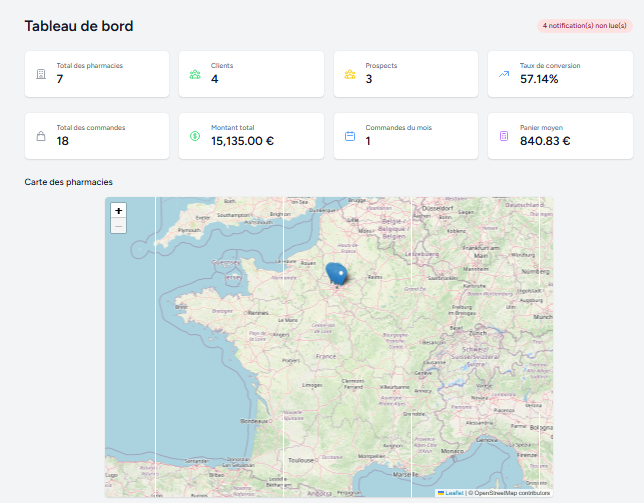
\includegraphics[width=0.8\textwidth]{Screens/1.0 - Base Tableau de bord Commerciaux.png}
\vspace{1cm}

\subsection*{Annexe 2 : 1.0 - Mauvaise disposition des graphiques}
\vspace{0.5cm}
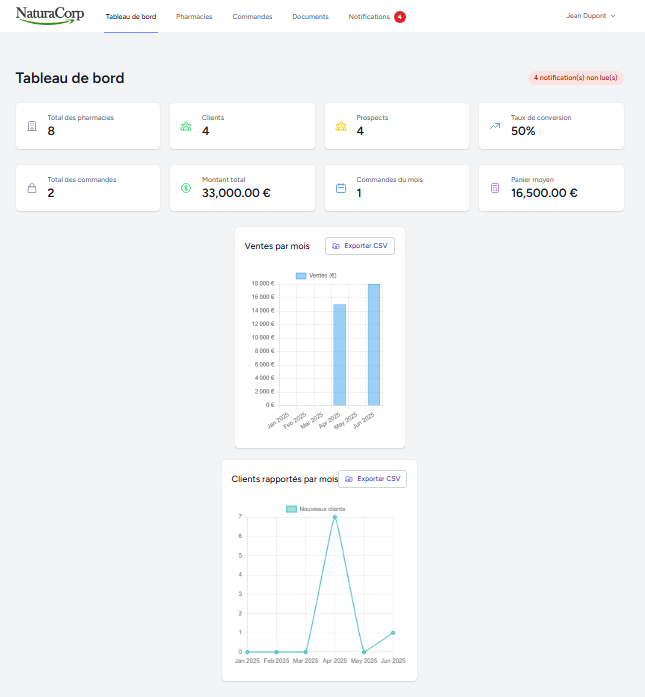
\includegraphics[width=0.8\textwidth]{Screens/1.0 - Mauvaise disposition des graphiques.png}
\vspace{1cm}

\subsection*{Annexe 3 : 1.5 - Graphiques Comerciaux Terminés}
\vspace{0.5cm}
\includegraphics[width=0.8\textwidth]{Screens/1.5 - Graphiques Comerciaux Terminés.png}
\vspace{1cm}

\subsection*{Annexe 4 : 2.0 - Base de la page rapport Admin}
\vspace{0.5cm}
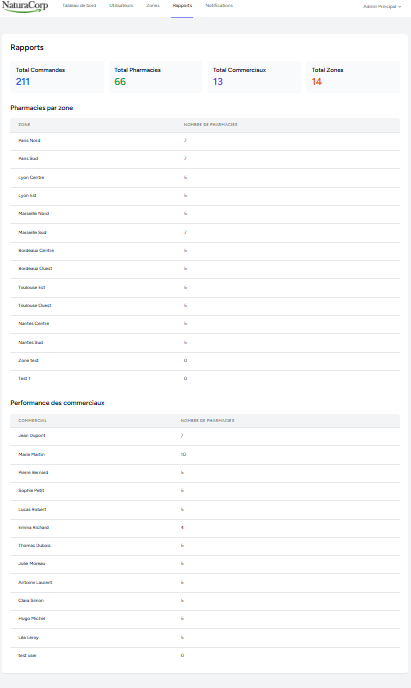
\includegraphics[width=0.8\textwidth]{Screens/2.0 - Base de la page rapport Admin.png}
\vspace{1cm}

\subsection*{Annexe 5 : 2.5 - Stats Admin pour zone}
\vspace{0.5cm}
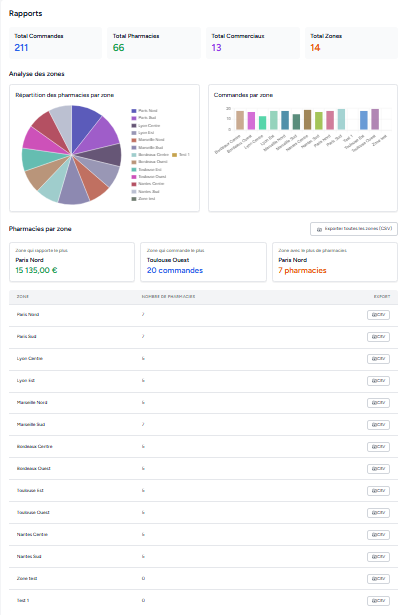
\includegraphics[width=0.8\textwidth]{Screens/2.5 - Stats Admin pour zone.png}
\vspace{1cm}

\subsection*{Annexe 6 : 2.5 - Stats admin pour commerciaux}
\vspace{0.5cm}
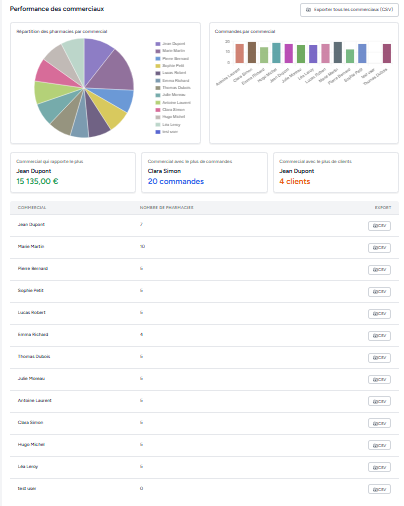
\includegraphics[width=0.8\textwidth]{Screens/2.5 - Stats admin pour commerciaux.png}
\vspace{1cm}


\end{document}
